\documentclass[10pt, conference, letterpaper]{IEEEtran}

\usepackage{graphicx}
\usepackage{amsmath}
\usepackage{amssymb}
\usepackage{booktabs}
\usepackage{cite}
\usepackage{subcaption}
\usepackage{algorithm}
\usepackage{algpseudocode}
\usepackage{url}

\graphicspath{{./figures/}}

\begin{document}

\title{Deep Reinforcement Learning for Snake: A PPO Implementation for a Snake Game Agent}
\IEEEoverridecommandlockouts
\author{Alexandru Mihailescu\thanks{Work done for the course of Reinforcement Learning, taught by Prof. Gian Antonio Susto at the University of Padua.}}

\maketitle

\begin{abstract}
This paper presents a deep reinforcement learning approach to the classic Snake game using Proximal Policy Optimization (PPO) with a custom convolutional neural network architecture. The agent learns to navigate a $10 \times 10$ grid, collecting fruits while avoiding collisions with walls and with its own body. Agent performance is studied under full and partial observability, and the impact of reward design is measured through a step penalty variant and a high-magnitude reward variant. The partially observable agent, restricted to a $5 \times 5$ local view, outperforms the fully observable one: it reaches a 7.2\% win rate and a 196\% improvement in mean episode reward over the heuristic baseline, which indicates that a smaller observation space can yield a policy that generalizes better. The best PPO agent clearly outperforms a heuristic iterative baseline, showing both the effectiveness of modern policy-gradient methods on discrete control tasks with sparse rewards and the sensitivity of the outcome to reward function design.
\end{abstract}

\section{Introduction}

The Snake game is a reinforcement learning problem in which the agent must maximize fruit collection while managing a continuously growing body. The body itself is a dynamic obstacle, so the problem combines navigation, planning, and self-avoidance in a discrete action space.

\subsection{Problem Formulation}

The Snake game is formulated as a Markov Decision Process (MDP) defined by the tuple $(\mathcal{S}, \mathcal{A}, \mathcal{P}, \mathcal{R}, \gamma)$:

\begin{itemize}
  \item State space $\mathcal{S}$: one-hot encoded board representation.
  \item Action space $\mathcal{A} = \{0, 1, 2, 3\}$: up, right, down, left.
  \item Transition $\mathcal{P}$: deterministic game mechanics.
  \item Reward $\mathcal{R}$: sparse rewards for fruit collection and penalties for collisions.
  \item Discount factor $\gamma = 0.99$.
\end{itemize}

\subsection{Environment Specification}

The environment is a $10 \times 10$ grid including walls, which yields an $8 \times 8$ playable area. The board is encoded as a one-hot tensor over the five cell categories (wall, empty space, fruit, body, head). The wall channel is dropped from the observation, so the tensor handed to the agent has shape $(H, W, 4)$.

\subsection{Observability Variants}

Two observation modes are investigated.

\textbf{Full observability}: the agent observes the complete $10 \times 10$ board state, which gives global information about fruit location and body positions.

\textbf{Partial observability}: the agent observes only a local $5 \times 5$ window centred on its head (mask size $= 2$), simulating a limited sensor range. This variant tests whether an effective policy can be learned from incomplete information.

\subsection{Critical Issues}

The Snake problem presents several reinforcement learning challenges.

\begin{itemize}
  \item \textbf{Sparse rewards}: positive feedback occurs only on fruit collection, which makes credit assignment difficult over long navigation sequences.
  \item \textbf{Growing complexity}: as the snake grows, the effective state space changes and becomes harder to navigate, and previously safe actions become dangerous. Filling almost the whole board requires near-perfect navigation with very little margin for error.
  \item \textbf{Self-trapping}: the agent can create board configurations from which no safe action exists, so long-term planning is essential.
  \item \textbf{Risk of reward hacking}: naive reward structures such as step penalties can incentivize unintended behaviour, for example early termination or endless oscillation in place.
\end{itemize}

\section{Reward Design}

Reward shaping changes learning dynamics. The default reward function shipped with the ready to use environment is designed to give a clear learning signal while limiting reward hacking. The agent receives $+1.0$ for filling the board (the win condition), $+0.5$ for collecting a fruit, $0.0$ for a normal step, $-0.2$ for a self-collision, and $-0.1$ for a wall collision.

\subsection{Step Penalty Variant}

A step penalty variant ($r_{\text{step}} = -0.001$) is tested to encourage efficient paths to the fruit. This reward was designed to force the agent into movement: early training runs produced agents that would "stand still" by moving left and right, or up and down, repeatedly. Charging a cost for every movement was meant to push the policy towards exploration in the direction of the fruit and towards better navigation strategies.

\subsection{High Penalty Variant}

The high penalty variant uses the reward values in Table~\ref{tab:rewards}. It was designed to strongly incentivize the win state of a completed board, while penalizing wall collision as harshly as self collision. The magnitudes are also higher than in the default reward set.

\begin{table}[t]
\centering
\caption{Reward function configurations tested.}
\label{tab:rewards}
\begin{tabular}{lrrr}
\toprule
Event & Default & Step Penalty & High Penalty \\
\midrule
Win            & 1.0  & 1.0    & 10.0 \\
Fruit          & 0.5  & 0.5    & 1.0 \\
Step           & 0.0  & -0.001 & 0.0 \\
Self-collision & -0.2 & -0.2   & -1.0 \\
Wall collision & -0.1 & -0.1   & -1.0 \\
\bottomrule
\end{tabular}
\end{table}

\section{Baseline Approach}

The performance baseline is a heuristic iterative agent that combines greedy path finding with survival checks. Algorithm~\ref{alg:baseline} gives the pseudo-code of the implementation.

\begin{algorithm}[t]
\caption{Greedy Baseline Agent}
\label{alg:baseline}
\begin{algorithmic}[1]
\Require observation $o$, head position $(h_x, h_y)$, fruit position $(f_x, f_y)$
\State Compute direction to fruit: $(\Delta x, \Delta y) = (f_x - h_x,\ f_y - h_y)$
\State Rank actions by: (1) moves toward fruit, (2) safe moves
\ForAll{action $a$ in ranked order}
  \State Simulate next position $(h_x', h_y')$
  \If{position is safe (not wall, not body)}
    \State \Return $a$
  \EndIf
\EndFor
\State \Return random safe action (or any action if none is safe)
\end{algorithmic}
\end{algorithm}

The baseline prioritizes moving toward the fruit while avoiding immediate death. It has no long-term planning and can trap itself in complex body configurations.

The greedy heuristic is a reasonable reference point because it encodes the intuitive human strategy: move toward the reward while avoiding immediate death. Its key limitation, the absence of planning into the future, leaves ample room for a learned policy to improve on it. A purely random baseline would be too weak, while planning algorithms derived from graph theory and path solving would set a very high, and possibly unreachable, ceiling for learning-based approaches under a limited computation budget. The greedy baseline sits in the middle and delivers consistent performance that a learning agent should be able to surpass.

\section{PPO Algorithm Design}

Proximal Policy Optimization (PPO) \cite{schulman2017ppo} is used. It is an actor-critic algorithm that combines sample efficiency with stable policy updates through a clipped surrogate objective.

\subsection{Algorithm Selection}

PPO was selected for the following reasons.

\begin{enumerate}
  \item \textbf{Discrete action space}: PPO handles discrete action spaces natively, as required here.
  \item \textbf{Sample efficiency}: compared with vanilla policy-gradient methods, PPO reuses collected trajectories across multiple epochs, which improves sample efficiency without the complexity of off-policy corrections and reduces exposure to the deadly triad.
  \item \textbf{Stable on-policy learning}: the clipped surrogate objective prevents large policy updates, which matters for the non-stationary reward structure of Snake, where early exploration looks very different from the late-game optimization the agent eventually needs. PPO is more stable than both A2C and DDPG, which makes it a good fit for discrete episodic tasks.
  \item \textbf{Computation limitations}: the Stable-Baselines3 \cite{raffin2021sb3} library used in this project offers a well-tested PPO implementation with vectorized environment support, so parallel training can make full use of the dedicated GPU available.
\end{enumerate}

DQN was considered as an alternative but would have required replay buffers and target networks, adding implementation complexity. Given the relatively simple discrete control structure of Snake, the balance of stability and efficiency in PPO made it the better choice.

\subsection{Policy Architecture}

The policy network uses a custom CNN feature extractor followed by separate policy and value heads. The architecture flows from a single input into the two output heads, and was diagrammed with PlotNeuralNet \cite{iqbal2018plotneuralnet}.

The input to the feature extractor is the one-hot encoded game state matrix of shape $(H, W, 4)$. Two $3 \times 3$ convolutions with padding 1 (32 then 64 channels, each followed by ReLU) are flattened and passed through a fully connected layer of 256 units. The policy head and the value head are each a 128-unit hidden layer on top of that shared feature vector, producing the four action logits and the scalar state value respectively. Table~\ref{tab:arch} lists the layers.

\begin{table}[t]
\centering
\caption{Feature extractor and heads.}
\label{tab:arch}
\begin{tabular}{lll}
\toprule
Stage & Layer & Output \\
\midrule
Input   & one-hot board            & $(H, W, 4)$ \\
Conv1   & Conv2d $3\times3$, pad 1 & 32 channels \\
Conv2   & Conv2d $3\times3$, pad 1 & 64 channels \\
FC      & Linear + ReLU            & 256 \\
Policy  & Linear + ReLU            & 128 $\rightarrow$ 4 \\
Value   & Linear + ReLU            & 128 $\rightarrow$ 1 \\
\bottomrule
\end{tabular}
\end{table}

\begin{figure}[t]
  \centering
  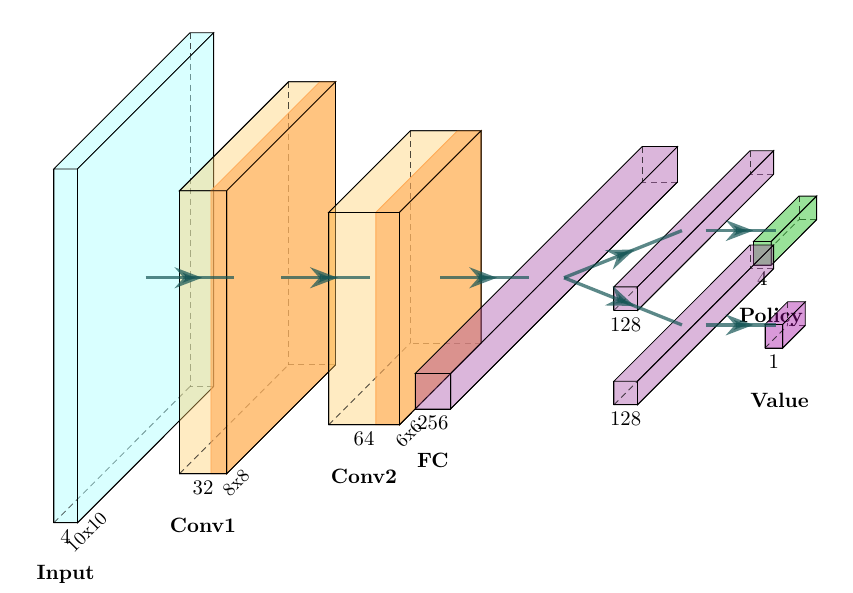
\includegraphics[width=\columnwidth]{network-architecture.png}
  \caption{Policy network. A shared convolutional feature extractor feeds separate policy and value heads.}
  \label{fig:arch}
\end{figure}

\subsection{PPO Objective}

The clipped surrogate objective prevents destructively large policy updates:

\begin{equation}
J(\theta) = \mathbb{E}_t \left[ \min \left( r_t(\theta) \, \hat{A}_t,\ \mathrm{clip}\left(r_t(\theta),\, 1 - \epsilon,\, 1 + \epsilon\right) \hat{A}_t \right) \right]
\end{equation}

where
\begin{equation}
r_t(\theta) = \frac{\pi_\theta(a_t \mid s_t)}{\pi_{\theta_{\text{old}}}(a_t \mid s_t)}
\end{equation}
is the probability ratio and $\hat{A}_t$ is the advantage estimated with Generalized Advantage Estimation (GAE).

The hyperparameters used for training are listed in Table~\ref{tab:hyper}. Relative to the Stable-Baselines3 defaults, the entropy coefficient of 0.01 encourages exploration during training, and the comparatively high number of epochs per batch allows thorough optimization of each collected trajectory. Mini-batch epochs were set to 15 and the number of parallel environments to 16 to make full use of the training rig.

\begin{table}[t]
\centering
\caption{Training hyperparameters.}
\label{tab:hyper}
\begin{tabular}{lr}
\toprule
Parameter & Value \\
\midrule
Total timesteps             & 6,000,000 \\
Parallel environments       & 16 \\
Learning rate               & $3 \times 10^{-4}$ \\
Discount factor             & 0.99 \\
GAE $\lambda$               & 0.9 \\
Clip range                  & 0.2 \\
Entropy coefficient         & 0.01 \\
Value function coefficient  & 0.5 \\
Batch size                  & 2048 \\
Mini-batch epochs           & 15 \\
Steps per rollout           & 1024 \\
Random seed                 & 0 \\
\bottomrule
\end{tabular}
\end{table}

\section{Implementation Details}

\subsection{Environment Unification}

The provided material contained two separate environment files, one for full observability and one for partial observability. These were merged into a single \texttt{environments.py} module with two modifications. First, both observability modes are reachable through a single mask size parameter: \texttt{None} or 0 for full observability, a positive integer for partial observability. The \texttt{to\_state()} function was adapted so that it returns the correct tensor in either mode. Second, a rewards dictionary parameter was added so that different reward values can be passed at construction time.

\subsection{Gymnasium Wrapper}

To use Stable-Baselines3, a custom Gymnasium wrapper (\texttt{gym\_environments.py}) adapts the merged environment to the library standard and exposes it to the PPO model. The wrapper enables integration with the vectorized environment utilities of SB3 (\texttt{SubprocVecEnv}), which is what allows parallel training across 16 environments and full GPU utilization on the training rig. Beyond the methods required by the Stable-Baselines3 documentation, the auxiliary \texttt{info} dictionary is used to supply additional signal during training: the distance from the head of the snake to the fruit, and the distance to the closest wall.

\section{Training}

\texttt{source/train\_ppo.py} implements the training of the PPO models from Stable-Baselines3. \texttt{train.py} drives a sequential process that trains all models across the different setups. Checkpoints are written every 200,000 timesteps as a safety measure, and training metrics (episode rewards and lengths) are logged for analysis.

Figure~\ref{fig:curves} shows the learning curves, computed as a 100-episode rolling average of episode reward over 6 million training steps. The model trained with the high penalty rewards shows the highest training reward. It does not generalize: as Table~\ref{tab:results} shows, it ends up only third best at evaluation. The baseline is shown for comparison, with a mean evaluation reward of 8.33.

\begin{figure}[t]
\centering
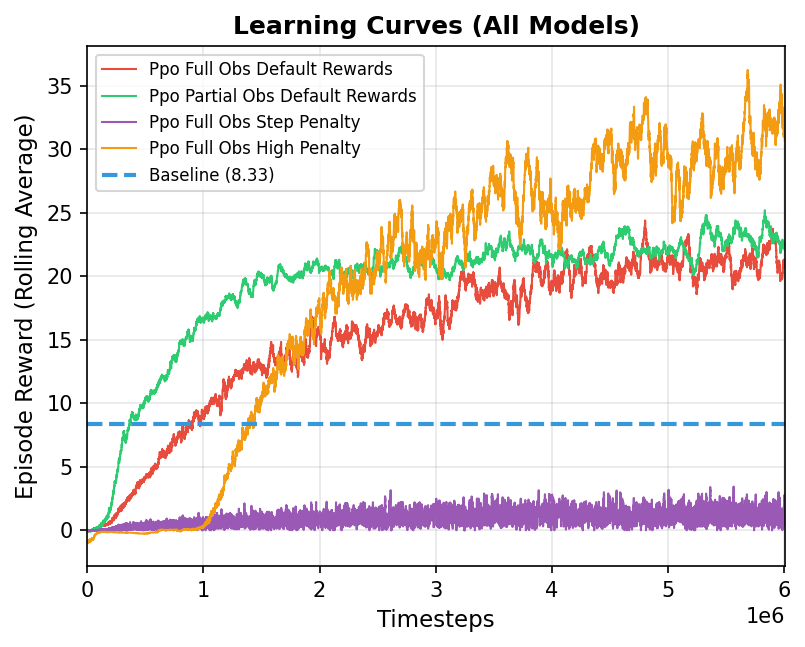
\includegraphics[width=\columnwidth]{learning_curves_all_models.png}
\caption{Learning curves for all PPO agent variants, with the baseline shown as a dashed horizontal line.}
\label{fig:curves}
\end{figure}

\section{Experimental Setup}

Four model variants are trained and evaluated.

\begin{enumerate}
  \item \textbf{Full observability, default rewards}: complete board visibility with the standard reward structure.
  \item \textbf{Partial observability, default rewards}: $5 \times 5$ local view with the standard rewards.
  \item \textbf{Full observability, step penalty}: complete visibility with the default rewards modified to include $r_{\text{step}} = -0.001$.
  \item \textbf{Full observability, high penalty}: complete visibility with high-magnitude rewards that incentivize wins, and an equal penalty for self-collision and wall collision.
\end{enumerate}

\begin{table}[t]
\centering
\caption{PPO agent improvements over the greedy baseline.}
\label{tab:improv}
\begin{tabular}{lrr}
\toprule
Agent & Reward & Improv. \\
\midrule
Full Obs      & +15.32 & +184\% \\
Partial Obs   & +16.29 & +196\% \\
Step Penalty  & -0.67  & -8\% \\
High Penalty  & +8.48  & +102\% \\
\bottomrule
\end{tabular}
\end{table}

\section{Results}

\subsection{Evaluation Protocol}

Each trained agent is evaluated over 500 episodes with a fixed seed (\texttt{seed=0}) for reproducibility. An episode terminates on collision, with a wall or with the body, or after a fixed maximum of 1000 time steps. Cumulative episode reward, number of fruits eaten, and win rate are collected during evaluation and saved. The baseline agent and all models are evaluated under identical environmental conditions, with the default reward values, so that the comparison between models is fair.

\subsection{Performance Comparison}

\begin{table}[t]
\centering
\caption{Evaluation results over 500 episodes.}
\label{tab:results}
\begin{tabular}{lrrr}
\toprule
Agent & Mean Reward & Mean Fruits & Win Rate \\
\midrule
Baseline      & 8.33 $\pm$ 2.43  & 17.07 $\pm$ 4.87  & 0.0\% \\
Full Obs      & 23.66 $\pm$ 9.09 & 47.70 $\pm$ 18.22 & 0.0\% \\
Partial Obs   & 24.63 $\pm$ 7.16 & 49.49 $\pm$ 14.02 & 7.2\% \\
Step Penalty  & 7.67 $\pm$ 12.07 & 15.47 $\pm$ 24.32 & 0.0\% \\
High Penalty  & 16.81 $\pm$ 9.04 & 33.98 $\pm$ 18.14 & 0.0\% \\
\bottomrule
\end{tabular}
\end{table}

\begin{figure}[t]
\centering
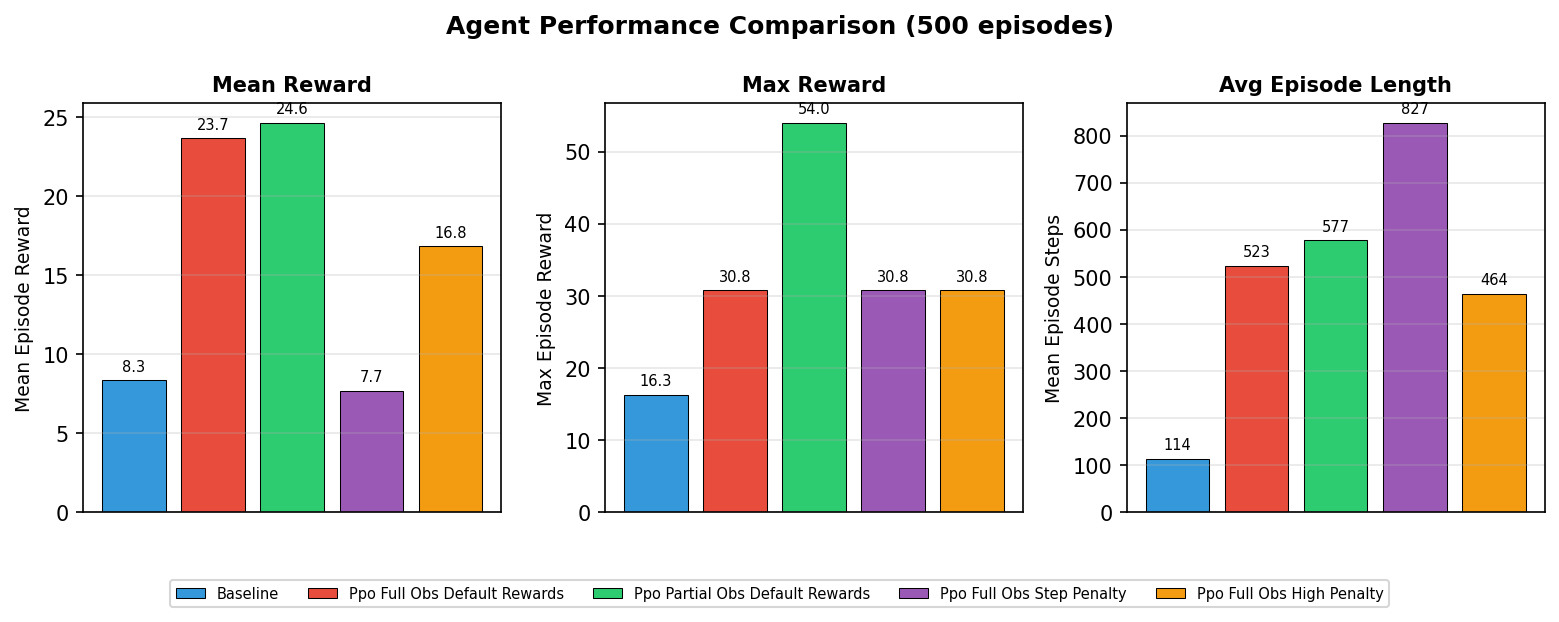
\includegraphics[width=\columnwidth]{performance_comparison.png}
\caption{Performance comparison across all agents.}
\label{fig:comparison}
\end{figure}

\begin{figure}[t]
\centering
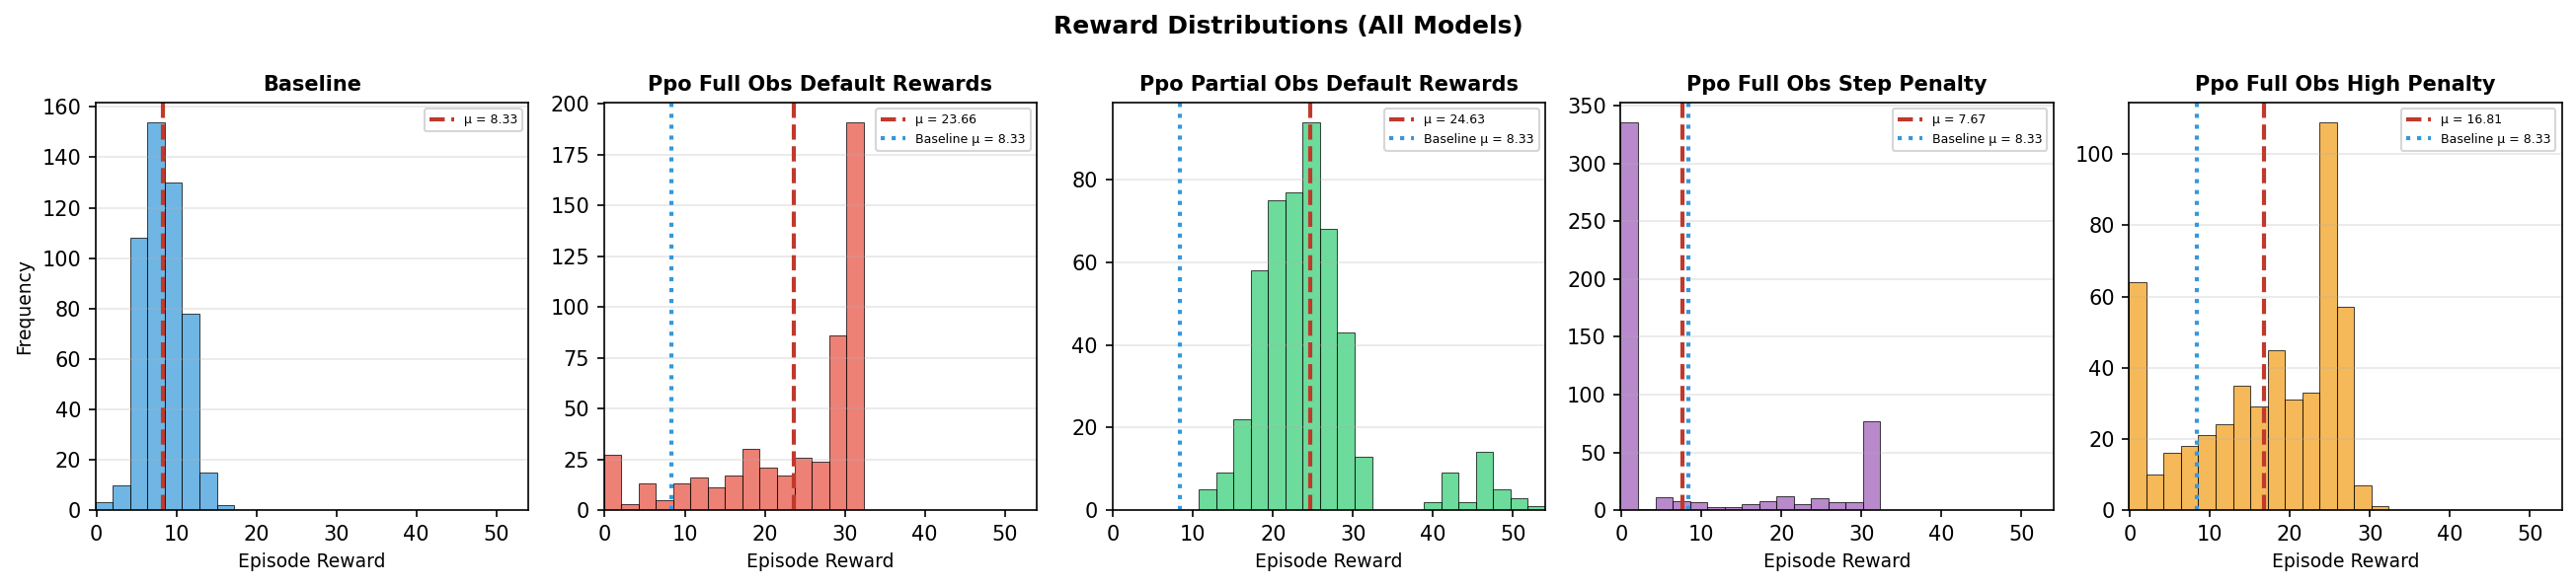
\includegraphics[width=\columnwidth]{reward_distributions.png}
\caption{Episode reward distributions during evaluation.}
\label{fig:dist}
\end{figure}

\subsection{Partial Observability Model}

Contrary to expectation, partial observability outperforms full observability on every metric (Table~\ref{tab:obs}). Several factors plausibly work in its favour. The dimensionality reduction of the local view makes the learning problem easier to solve within the same computation budget. The restricted view also acts as a noise filter, hiding cells that are not relevant at the current moment. The partially observable model has the best mean reward per episode, and it is the only model that achieves wins at all (7.2\%), which also indicates good navigation in late-game configurations. It is likewise the only model that never died before eating at least 20 fruits across the 500 evaluation episodes (Fig.~\ref{fig:dist}), in contrast with every other reward experiment.

\begin{table}[t]
\centering
\caption{Full versus partial observability, default rewards.}
\label{tab:obs}
\begin{tabular}{lrrr}
\toprule
Metric & Full Obs & Partial Obs & Difference \\
\midrule
Mean Reward & 23.66 & 24.63 & +4.1\% \\
Std Reward  & 9.09  & 7.16  & -21.2\% \\
Max Reward  & 30.80 & 54.00 & +75.3\% \\
Win Rate    & 0.0\% & 7.2\% & +7.2\% \\
\bottomrule
\end{tabular}
\end{table}

\begin{figure}[t]
\centering
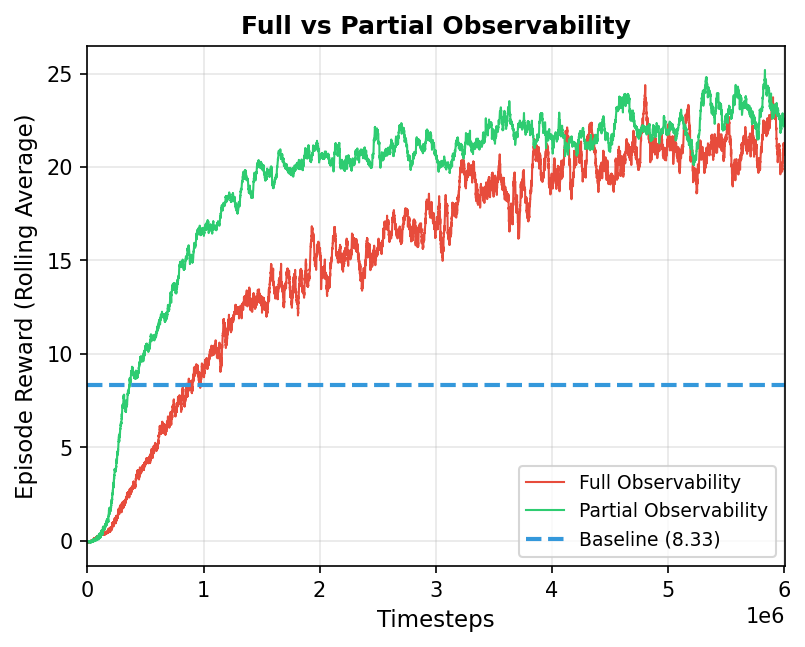
\includegraphics[width=\columnwidth]{full_vs_partial_observability.png}
\caption{Learning curves comparing full ($10\times10$) and partial ($5\times5$) observability. Despite reduced information, partial observability converges faster and reaches higher final performance.}
\label{fig:fullpartial}
\end{figure}

\subsection{Reward Value Experiments}

\textbf{Default rewards.} The default reward configuration generalizes best. Both the full and the partial observability models improve by 10 to 11\% from training to evaluation, and by more than 184\% over the greedy baseline. These models also reach the highest mean reward per episode of all trained models.

\textbf{Step penalty.} The step penalty model performs worse than the baseline ($-8\%$) even though it improves from training to evaluation (Table~\ref{tab:trainval}). The step penalty creates conflicting incentives: fruit rewards encourage survival while step penalties penalize it. Over 1000 steps the cumulative step penalty ($-1.0$) exceeds two fruit rewards, so the policy learns immediate self-termination. This is visible in Fig.~\ref{fig:dist}, where more than 60\% of episodes score 0.0. As Fig.~\ref{fig:curves} shows, the step penalty model also learned very slowly, with an average reward across the 6 million timesteps well below the iterative baseline. Penalties that conflict with the survival objective can destabilize learning catastrophically.

\begin{table}[t]
\centering
\caption{Training versus evaluation performance.}
\label{tab:trainval}
\begin{tabular}{lrr}
\toprule
Agent & Train mean ep. reward & Eval mean ep. reward \\
\midrule
Full Obs     & 21.23 & 23.66 \\
Partial Obs  & 22.39 & 24.63 \\
High Pen.    & 30.70 & 16.81 \\
Step Pen.    & 0.46  & 7.67 \\
\bottomrule
\end{tabular}
\end{table}

\textbf{High penalty.} Despite the highest training reward, the high penalty model drops 45.2\% from training to evaluation, which indicates severe overfitting. It generally performs well, with an average episode reward close to that of the fully observable default rewards model, but it also produces a large number of episodes scoring 0, as seen in Fig.~\ref{fig:dist}. The higher win and fruit rewards appear to have a positive impact on maximum and average reward, while the higher self-collision and wall-collision penalties have a negative effect, producing a higher reward variance per episode than the default set of rewards.

\section{Discussion}

The results confirm that a reinforcement learning algorithm such as PPO can substantially outperform a heuristic iterative algorithm. Counter to intuition, partial observability can be advantageous in this setting, improving performance across the board relative to full observability. Reward shaping needs careful design: rewards can stunt learning outright, as the step penalty experiment shows, and high-magnitude rewards can cause overfitting. Moderate, balanced rewards (the default configuration) generalize best.

\subsection{Limitations}

\begin{itemize}
  \item \textbf{Fixed board size}: models were trained and evaluated only on $10 \times 10$ boards. Generalization to other sizes is untested.
  \item \textbf{Computational cost}: training ran for 6 million timesteps (roughly 3 to 5 minutes per model with CUDA support). The total hours spent on training and experimentation, from start to finish of the project, were substantial even on a mid-range GPU. As board size grows, the computational cost of reaching comparable performance should be expected to grow steeply, along with the complexity of the problem to be learned.
  \item \textbf{Win rate ceiling}: even the best model reaches only 7.2\% wins, so the late-game problem remains challenging.
\end{itemize}

\section{Conclusion}

A PPO agent applied to the 2D Snake game substantially outperforms a heuristic baseline, and the experiments challenge two conventional assumptions.

\begin{enumerate}
  \item Partial observability can be an advantage. Here it enabled better generalization through an improved signal-to-noise ratio.
  \item Reward shaping requires careful design. Step penalties can create conflicting incentives that lead to policy collapse, and high-magnitude rewards can cause overfitting and high variance in behaviour.
\end{enumerate}

\subsection{Future Work}

\begin{itemize}
  \item Curriculum learning with increasing board sizes, to improve late-game performance.
  \item A larger computation budget, to find the limits of the models under the current implementation.
  \item Action masking, to prevent invalid moves and improve sample efficiency.
\end{itemize}

\bibliographystyle{IEEEtran}
\bibliography{biblio}

\end{document}
